\documentclass[a4paper,german,12pt,smallheadings]{scrartcl}
\usepackage[T1]{fontenc}
\usepackage[utf8]{inputenc}
\usepackage{babel}
\usepackage{geometry}
\usepackage[fleqn]{mathtools} % also includes mathclap
\usepackage[fleqn]{amsmath}
\usepackage{amssymb}
\usepackage{float}
\usepackage{enumerate}
\usepackage{commath} % http://tex.stackexchange.com/questions/14821/whats-the-proper-way-to-typeset-a-differential-operator
\usepackage{cancel}

% Number only referenced equations
\mathtoolsset{showonlyrefs}

%\usepackage{wrapfig}
\usepackage[thinspace,thinqspace,squaren,textstyle]{SIunits}

% New command for color underlining
\usepackage{xcolor}

\newsavebox\MBox
\newcommand\colul[2][red]{{\sbox\MBox{$#2$}%
  \rlap{\usebox\MBox}\color{#1}\rule[-1.2\dp\MBox]{\wd\MBox}{0.5pt}}}

\restylefloat{table}
\geometry{a4paper, top=15mm, left=10mm, right=20mm, bottom=20mm, headsep=10mm, footskip=12mm}
\linespread{1.2}
\setlength\parindent{0pt}
\DeclareMathOperator{\Tr}{Tr}
\DeclareMathOperator{\Var}{Var}
\newcommand*\laplace{\mathop{}\!\mathbin\Delta}
\begin{document}
\allowdisplaybreaks % Seitenumbrüche in Formeln erlauben
\begin{center}
\bfseries % Fettdruck einschalten
\sffamily % Serifenlose Schrift
\vspace{-40pt}
Theoretische Elektrodynamik, Sommersemester 2014, Aufgabenblatt 8

Markus Fenske, Mattis Riediger, Tutor: Clemens Meyer zu Rheda
\vspace{-10pt}
\end{center}

\section*{Aufgabe 1: Zylinderspule}
\begin{enumerate}[a)]
\item
Mit dem Biot-Savart-Gesetz
\begin{equation}
  \vec{B}(\vec{r}) = \frac{\mu_0}{4 \pi} \int \dif V' \; \vec{j}(\vec{r}) \times
  \frac{\vec{r} - \vec{r}'}{\envert{\vec{r} - \vec{r}'}^3}
\end{equation}

und der gegebenen Stromverteilung
\begin{equation}
  \vec{j} = I n \hat{e}_\varphi \delta(r_\perp - R) \del{
    \Theta(z+L) - \Theta(z-L)
  }
\end{equation}

erhalten wir in Zylinderkoordinaten für das Feld auf der $z$-Achse ($\vec{r} =
z \hat{e}_z$):
\begin{align*}
  \vec{B}(z)
  &= \frac{\mu_0}{4 \pi}
  \int\limits_0^{2 \pi} \dif \varphi'
  \int\limits_{-\infty}^{\infty} \dif z'
  \int\limits_{0}^{\infty} \dif r' \;
  r'
  I n \hat{e}_\varphi \delta(r' - R) \del{
    \Theta(z+L) - \Theta(z-L)
  }
  \times
  \frac{
    z \hat{e_z} - (z' \hat{e}z + r' \hat{e}_r)
  }{
    \sqrt{(z-z')^2 + r'^2}^3
  } \\
  &= \frac{\mu_0}{4 \pi}
  \int\limits_0^{2 \pi} \dif \varphi'
  \int\limits_{-L}^{L} \dif z' \;
  R
  I n \hat{e}_\varphi
  \times
  \frac{
    (z-z') \hat{e_z} - R \hat{e}_r
  }{
    \sqrt{(z-z')^2 + R^2}^3
  } \\
  &= \frac{\mu_0 R I n}{4 \pi}
  \int\limits_0^{2 \pi} \dif \varphi'
  \int\limits_{-L}^{L} \dif z' \;
  \del{
    \frac{
      (z-z') (\hat{e}_\varphi \times \hat{e_z})
    }{
      \sqrt{(z-z')^2 + R^2}^3
    }
    -
    \frac{
      R (\hat{e}_\varphi \times \hat{e}_r)
    }{
      \sqrt{(z-z')^2 + R^2}^3
    }
  } \\
  &= \frac{\mu_0 R I n}{4 \pi}
  \int\limits_0^{2 \pi} \dif \varphi'
  \int\limits_{-L}^{L} \dif z' \;
  \del{
    \frac{
      (z-z') \hat{e_r}
    }{
      \sqrt{(z-z')^2 + R^2}^3
    }
    +
    \frac{
      R \hat{e}_z
    }{
      \sqrt{(z-z')^2 + R^2}^3
    }
  }
\end{align*}

Wegen $
  \int\limits_0^{2 \pi} \dif \varphi \; \hat{e}_r =
  \int\limits_0^{2 \pi} \dif \varphi \; \begin{pmatrix}
    \cos \varphi \\
    \sin \varphi \\
  \end{pmatrix}
  = 0
$
verschwindet der erste Term. Der zweite Term ist $\varphi$-invariant, also

\begin{align*}
  \vec{B}(z)
  &= \frac{\mu_0 R I n}{2}
  \int\limits_{-L}^{L} \dif z' \;
  \frac{
    R \hat{e}_z
  }{
    \sqrt{(z-z')^2 + R^2}^3
  }
\end{align*}

Mit der Substitution $x(z') = z - z'$, $\dif x = - \dif z'$ wird das zu

\begin{align*}
  \vec{B}(z)
  &= -\frac{\mu_0 R^2 I n}{2} \hat{e}_z
  \int\limits_{z+L}^{z-L} \dif x \;
  \frac{
    1
  }{
    \sqrt{x^2 + R^2}^3
  } \\
  &= -\frac{\mu_0 R^2 I n}{2} \hat{e}_z
  \sbr[3]{
    \frac{x}{R^2 \sqrt{x^2 + R^2}}
  }_{x=z+L}^{x=z-L} \\
  &= -\frac{\mu_0 I n}{2} \hat{e}_z
  \del{
    \frac{z-L}{\sqrt{(z-L)^2 + R^2}}
    -\frac{z+L}{\sqrt{(z+L)^2 + R^2}}
  } \\
  &= \frac{\mu_0 I N}{4L} \hat{e}_z
  \del{
    \frac{L-z}{\sqrt{(L-z)^2 + R^2}}
    +\frac{L+z}{\sqrt{(L+z)^2 + R^2}}
  }
\end{align*}
% FIXME: Bah, sieht dieses Mathematica hässlich aus. Machen wir mit PGFplot
% neu, wenn noch Zeit.
\item Siehe Abbildung 1.
  \begin{figure}[h!]
    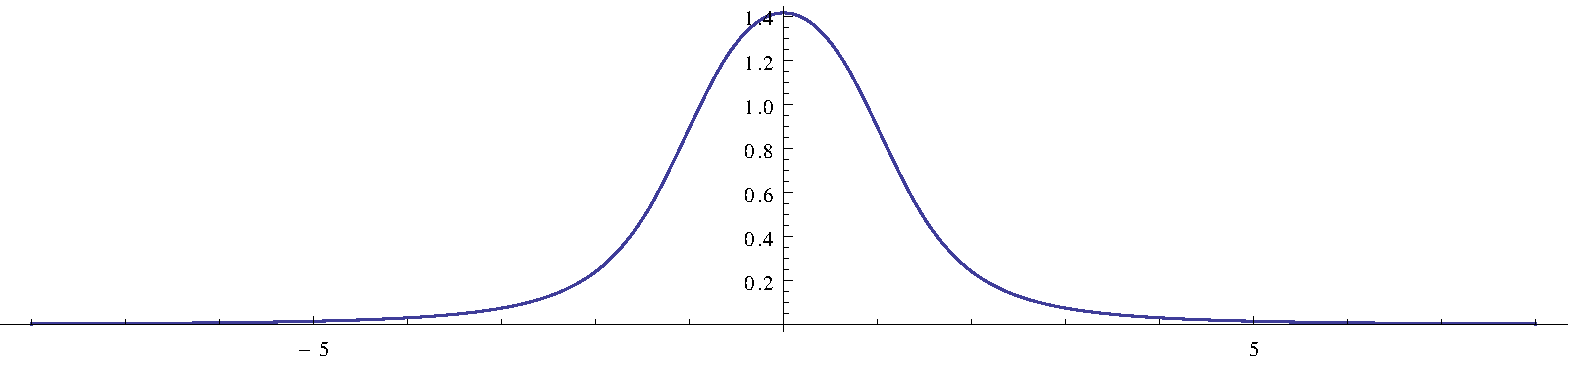
\includegraphics[width=\textwidth]{plot-zylinderspule.pdf}
    \label{zylinderspule}
    \caption{Magnetfeld $\vec{B}(z) = B \hat{e}_z$ einer Zylinderspule.}
  \end{figure}
\end{enumerate}
\end{document}
